% This is samplepaper.tex, a sample chapter demonstrating the
% LLNCS macro package for Springer Computer Science proceedings;
% Version 2.21 of 2022/01/12
%
\documentclass[runningheads]{llncs}
%
\usepackage[T1]{fontenc}
% T1 fonts will be used to generate the final print and online PDFs,
% so please use T1 fonts in your manuscript whenever possible.
% Other font encondings may result in incorrect characters.
%
\usepackage{graphicx}
\usepackage{caption}
\usepackage{float}
\usepackage{algorithm}
\usepackage{algpseudocode}
\usepackage{amsmath} % Para el comando \text si es necesario, aunque en este caso no lo es directamente para el pseudocódigo.
\usepackage{graphicx}
% Used for displaying a sample figure. If possible, figure files should
% be included in EPS format.
%
% If you use the hyperref package, please uncomment the following two lines
% to display URLs in blue roman font according to Springer's eBook style:
%\usepackage{color}
%\renewcommand\UrlFont{\color{blue}\rmfamily}
%\urlstyle{rm}
%
\begin{document}
%
\title{Genetic Algorithm for Bayesian Network Structure Learning: Evaluation on Benchmark and Synthetic Datasets}

%\titlerunning{Abbreviated paper title}
% If the paper title is too long for the running head, you can set
% an abbreviated paper title here
%
\author{Angel García Báez\inst{1}\inst{2} }
%
\authorrunning{Angel García Báez.}
% First names are abbreviated in the running head.
% If there are more than two authors, 'et al.' is used.
%
\institute{Universidad Veracruzana, Veracruz, México \and
Instituto de Investigaciones en Inteligencia Artificial, Veracruz, Mexico
\email{zs24013216@estudiantes.uv.mx}\\
\url{https://www.uv.mx/iiia/} }
%
\maketitle              % typeset the header of the contribution
%
\begin{abstract}
Abstract Pendiente
\keywords{Bayesian networks, Genetic algorithms, Structure learning, Minimum description length, UCI datasets, KL divergence, Structural Hamming Distance}
\end{abstract}

%
%
%
\section{Introduction}

Bayesian networks (BNs) are compact probabilistic graphical models representing joint probability distributions and conditional dependencies between random variables by a directed acyclic graph (DAG). Causal modeling ability makes them useful in medical, financial, and bioinformatics domains. The larger the number of variables, the harder learning the structure of a BN from data is. This is partly because of the combinatorial explosion of graph structures that are possible, a problem which is shown to be NP-hard [Chickering, 1996].

Conventional structure learning methods can be categorized as score-based, constraint-based, and hybrid. Score-based methods utilize search algorithms that are informed by scores such as MDL (Minimum Description Length), BIC (Bayesian Information Criterion), or BDeu (Bayesian Dirichlet Equivalent Uniform) to assess candidate structures. While these are sound methods, their efficiency declines considerably with the rise in dimensionality and intricacy of the data.

Over the past several years, heuristic and metaheuristic algorithms have been investigated to break through these constraints. Evolutionary computation methods, including genetic algorithms (GAs), have been very successful in optimizing BN structures in high-dimensional spaces. For example, the paper by Zhang et al. [1] presents an enhanced genetic algorithm that develops a novel crossover operator and outperforms traditional methods.

Additionally, hybrid models such as the adaptive Bayesian network model introduced by Rosendo et al. [2] integrate adaptive mechanisms into the evolutionary process so that the algorithm can adapt operators dynamically according to feedback from the search process. These directions of research provide interesting opportunities for extending BN learning to more complicated datasets.

Due to its significance and challenge in BN structure learning, this paper proposes a genetic algorithm-based approach that incorporates acyclicity checking and MDL-based scoring. The proposed approach is evaluated on some UCI data and gold standard networks to validate its efficacy in terms of both accuracy and structural faithfulness.



\section{Related Work/Background}


Bayesian networks have long been a powerful tool for modeling probabilistic relationships and reasoning under uncertainty. However, one of the key challenges in this domain lies in learning the structure of these networks from data, a task that is known to be NP-hard \cite{chickering1996learning}. Over the years, numerous approaches have been proposed to tackle this problem, ranging from greedy search strategies to more sophisticated metaheuristic methods.

One line of research focuses on optimizing score-based functions, where the goal is to find the structure that best fits the data according to a criterion such as MDL, BIC, or BDeu. In this context, Sun and Zhou \cite{sun2022bayesian} introduced an improved genetic algorithm that incorporates a novel biased crossover operator. This operator encourages the inheritance of promising substructures while maintaining diversity through random mutations and selective pressure. Their work demonstrates significant improvements over traditional genetic strategies in terms of convergence and quality of the learned networks.

Together, these works provide the theoretical and practical foundation for the methodology developed in this study. We draw inspiration from both: adopting the crossover strategy from \cite{sun2022bayesian}, and maintaining the modular flexibility and adaptive potential.


\newpage

\section{Proposed Method}

\subsection{Chromosome Representation}

Each individual in the population is represented as a numerical vector of length $p^2$, where p is the number of variables in the data set. This vector contains in its interior continuous random values between 0 and 1 at each position, so that it simulates the probability of existence of a directed edge between each pair of nodes of the network.

This vector is transformed by a threshold (defined by default at 0.5 by ~\cite{sun2022bayesian}) to convert each value into a binary number representing the presence or absence of a directed connection between 2 variables (nodes) of the network. Such a binarized vector is converted into a matrix of size $p\times p$ representing the adjacency matrix of a possible network structure.
To ensure that the adjacency matrix is free of cycles, a cycle detection function based on a depth search is implemented to identify and eliminate edges that generate cycles in the network.

\subsection{Initial Population Generation}

The initial population is randomly generated as a list of pobsize vectors with uniform random elements ranging from [0,1] that will be decoded and checked for cyclicity problems.


\begin{figure}[h!]
	\centering
	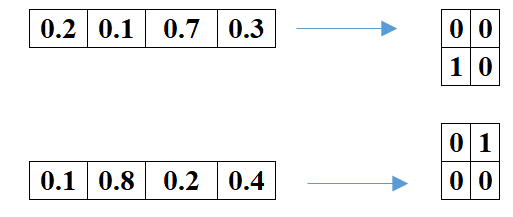
\includegraphics[width=0.7\linewidth]{IMG/P1}
	\caption{Representation of vector to adyacent matrix.}
	\label{fig:p1}
\end{figure}

\subsection{Fitness Function: MDL Scoring}

The objective function to be minimized corresponds to the MDL criterion. This is calculated as the sum of the model complexity and the negative likelihood of the data fitted to the proposed structure. A frequency count approach is used for categorical data. The resulting structure is evaluated with respect to the original data set train partition and a MDL score is assigned to each individual.

\subsection{Genetic Operators}

The implementation of the genetic operators is inspired by the scheme proposed in the paper “Bayesian Network Structure Learning: An Improved Genetic Algorithm Based on a New Crossover Operator”. The general flow of the genetic algorithm follows a modular structure based on three main operators:

\subsubsection{Selection}

Selection: elitist selection is used, where a fixed percentage of the best individuals are retained according to their MDL. This strategy ensures that the best solution found so far is not lost in future generations. Whatever the percentage of elitism and the size of the population, individuals are preserved.

\subsubsection{Biased Crossover}

A biased recombination operator with probability chooses genes from the elite or non-elite individual, thus allowing a balance between exploitation (inheriting promising structures) and exploration (introducing variability).

\subsubsection{Mutation}

New, completely random individuals are generated. These mutants represent a form of reinjection of genetic diversity into the evolutionary process, avoiding premature convergence of the algorithm.

\subsection{Generation Cycle}

Each new generation is composed of three groups: preserved elites, crossbred offspring and random mutants. The division allows the strengths of different search strategies to be exploited:

\begin{itemize}
	\item Elites ensure that the best solutions remain unmodified.
	\item Offspring explore new combinations based on the previous best individuals.
	\item Mutants introduce new evolutionary trajectories not dependent on the past.		
\end{itemize}


\begin{algorithm}
	\caption{Genetic Algorithm for Bayesian Network Learning}
	\label{alg:genetic_bn_learning_simple}
	\begin{algorithmic}[1]
		\Require Data ($D$, categorical)
		\Require $N_{gen}$ (Number of generations)
		\Require $P_{size}$ (Population size)
		\Require $p_e$ (Elite proportion)
		\Require $p_m$ (Mutation proportion)
		\Require $\rho$ (Biased crossover probability)
		\Ensure Best Bayesian Network structure (adjacency matrix)
		
		\State Initialize population of size $P_{size}$ with random vectors.
		\State Evaluate initial population using \textbf{MDL} (Minimum Description Length).
		\For{generation = 1 to $N_{gen}$}
		\State Select elite individuals ($p_e \times P_{size}$).
		\State Generate children via biased crossover ($\rho$).
		\State Generate random mutants ($p_m \times P_{size}$).
		\State Form new population: elites + children + mutants.
		\State Decode and enforce acyclicity for all individuals.
		\State Evaluate fitness (\textbf{MDL}) for new population.
		\EndFor
		\State \Return Individual with best \textbf{MDL}.
	\end{algorithmic}
\end{algorithm}



\newpage

\section{Experimental Setup}

\subsection{Hardware and software}

All experiments were performed on a laptop equipped with an Intel Core i5-12450H processor at 2.0 GHz, 16 GB of DDR5 RAM at 4800 MHz and 64-bit operating system. The development environment used was the R programming language, supported mainly by the bnlearn library for parameter setting of Bayesian Networks.

\subsection{Datasets for learning structure}

Ten data sets of diverse nature were used to validate the performance of the genetic algorithm taken from UCI machine learning repository. The following table summarizes their main characteristics:

\begin{table}[h!]
	\centering
	\caption{Dataset for Learning its Structure}
	\begin{tabular}{|c|c|c|c|}
		\hline
		\textbf{Index} & \textbf{Dataset} & \textbf{Variables} & \textbf{Instances} \\
		\hline
		1 & Iris & 4 & 150 \\
		\hline
		2 & PalmerPenguin & 4 & 342 \\
		\hline
		3 & Vinos & 13 & 178 \\
		\hline
		4 & HeartAttack & 13 & 297 \\
		\hline
		5 & CarsEvaluation & 6 & 1728 \\
		\hline
		6 & MaternalHealthRisk & 7 & 1014 \\
		\hline
		7 & Raisins & 7 & 900 \\
		\hline
		8 & Nurserys & 8 & 12960 \\
		\hline
		9 & Glass & 9 & 214 \\
		\hline
		10 & Zoo & 17 & 101 \\
		\hline
	\end{tabular}
\end{table}

\subsection{Golden networks}

Additionally, seven publicly available Bayesian reference networks (“gold networks”) were employed in bnlearn format. These networks were used to generate 1000 synthetic instances by simulation with the rbn function. Then, the genetic algorithm was applied on these data to learn their underlying structure. The networks included were: ASIA, CANCER, EARTHQUAKE, SACHS, SURVEY, CHILD and INSURANCE.

\begin{table}[h!]
	\centering
	\caption{Golden Networks Characteristics}
	\begin{tabular}{|l|c|c|c|}
		\hline
		\textbf{Golden Network} & \textbf{Nodes} & \textbf{Arcs} & \textbf{Parameters} \\
		\hline
		ASIA & 8 & 8 & 18 \\
		\hline
		CANCER & 5 & 4 & 10 \\
		\hline
		EARTHQUAKE & 5 & 4 & 10 \\
		\hline
		SACHS & 11 & 17 & 178 \\
		\hline
		SURVEY & 6 & 6 & 21 \\
		\hline
		CHILD & 20 & 25 & 230 \\
		\hline
		INSURANCE & 27 & 52 & 1008 \\
		\hline
	\end{tabular}
\end{table}

\subsection{Data preprocesing}

All data sets were preprocessed as follows:

\begin{itemize}
	\item Numerical variables were discretized if necessary by making use of the manually implemented CAIMD method.
	
	\item Subsequently, all columns were converted into categorical variables (factors).

	\item This transformation is crucial to ensure compatibility with the implemented CDM calculation model based on frequency counts.
	
\end{itemize}

\subsection{Genetic algorithm parameters}

The parameters used for the genetic algorithm in all experiments were as follows:

\begin{itemize}
	\item Number of generations: \textbf{50}
	\item Population size: \textbf{30}
	\item Elitism percentage: \textbf{20\%}
	\item Mutation percentage: \textbf{20\%}
	\item Binarization threshold: \textbf{0.5}
	\item Probability of elite inheritance in crossover: \textbf{0.7}
\end{itemize}

\subsection{Metrics}

For the datasets from the UCI Machine Learning Repository, an 80\% partition was used for structure learning and parameter fitting, while the remaining 20\% was reserved for accuracy evaluation. For each dataset, three metrics are reported: MDL (Minimum Description Length), accuracy, and computational time in seconds.

On the other hand, 7 known golden networks (Asia, Cancer, Earthquake, Sachs, Survey, Child, Insurance) were used. For each of these, 1000 synthetic instances were generated using \texttt{bnlearn}, and subsequently, the genetic algorithm was applied to infer their structure from this data. Finally, the inferred networks were compared against the true networks using two metrics:

\begin{itemize}
	\item \textbf{Kullback-Leibler Divergence:}.
	
	\begin{equation}
		D_{\text{KL}}(P \parallel Q) = \sum_{x} P(x) \log \frac{P(x)}{Q(x)}
	\end{equation}
	
	\item \textbf{Structural Difference:}.
	\begin{equation}
		SHD(G_1, G_2) = \text{Number of edge additions, deletions, and reversals to convert } G_1 \text{ into } G_2
	\end{equation}
	
	
\end{itemize}


\newpage

\section{Results}

\subsection{Evaluation on UCI Benchmark Datasets}

The proposed genetic algorithm was evaluated on ten benchmark datasets from the UCI repository. Each dataset was split using an 80\%/20\% scheme: 80\% was used to learn the Bayesian network structure and estimate the conditional probability tables (CPTs), while the remaining 20\% served for testing the classification accuracy.
Table~\ref{tab:uci_results} summarizes the Minimum Description Length (MDL), classification accuracy, and total computation time for each dataset. The results reflect the algorithm’s ability to adapt to datasets with varying sizes, complexity, and number of classes.

\begin{itemize}
	\item \textbf{Iris and PalmerPenguin:} Both with 4 variables and 3 classes, achieved high accuracy (93.3\% and 95.6\%, respectively) with low MDL and short computation times under 16 seconds.
	\item \textbf{The Wine dataset:} With 13 variables, yielded the highest accuracy (97.2\%) but required more computation time (93.6s), highlighting the trade-off between dimensionality and convergence time.
	\item \textbf{HeartAttack and MaternalHealthRisk:} While moderately complex, showed lower accuracies (72.9\% and 65\%) and higher MDL scores, suggesting challenges in capturing the underlying structure.
	\item \textbf{CarsEvaluation:} Despite its larger number of instances (1728), attained good classification performance (87.9\%) with a moderate MDL.
	\item \textbf{The most computationally intensive case was Nurserys:} It has over 12,000 instances and 5 classes. It achieved 92\% accuracy but incurred the highest MDL value and the longest training time (187.4s).
	\item \textbf{Glass and Zoo:} Both with more variables and classes, delivered satisfactory results, with the Zoo dataset reaching 100\% accuracy, albeit with a relatively high MDL.
\end{itemize}

\begin{table}[htbp]
	\centering
	\caption{Performance of the genetic algorithm on UCI datasets}
	\begin{tabular}{|c|l|c|c|c|c|c|c|}
		\hline
		\textbf{Index} & \textbf{Dataset} & \textbf{Variables} & \textbf{Instances} & \textbf{Classes} & \textbf{MDL} & \textbf{Accuracy (\%)} & \textbf{Time (s)} \\
		\hline
		1  & Iris                & 4  & 150   & 3 & 574.95      & 93.3 & 14.57  \\
		2  & PalmerPenguin       & 4  & 342   & 3 & 1123.32     & 95.6 & 15.80  \\
		3  & Wine                & 13 & 178   & 3 & 2211.30     & 97.2 & 93.64  \\
		4  & HeartAttack         & 13 & 297   & 2 & 3228.68     & 72.9 & 174.23 \\
		5  & CarsEvaluation      & 6  & 1728  & 3 & 15757.02    & 87.9 & 60.97  \\
		6  & MaternalHealthRisk  & 7  & 1014  & 3 & 5927.63     & 65.0 & 75.43  \\
		7  & Raisins             & 7  & 900   & 2 & 3258.89     & 87.2 & 90.26  \\
		8  & Nurserys            & 8  & 12960 & 5 & 146373.34   & 92.0 & 187.42 \\
		9  & Glass               & 9  & 214   & 7 & 3241.74     & 75.7 & 109.75 \\
		10 & Zoo                 & 17 & 101   & 7 & 1003.95     & 100.0& 169.06 \\
		\hline
	\end{tabular}
	\label{tab:uci_results}
\end{table}

\begin{figure}[htbp]
	\centering
	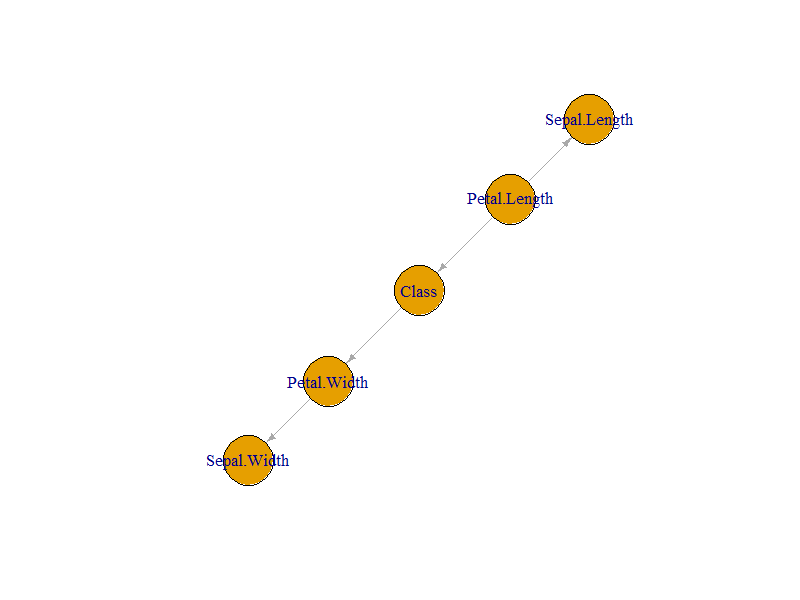
\includegraphics[width=0.4\textwidth]{IMG/1RED.png}
	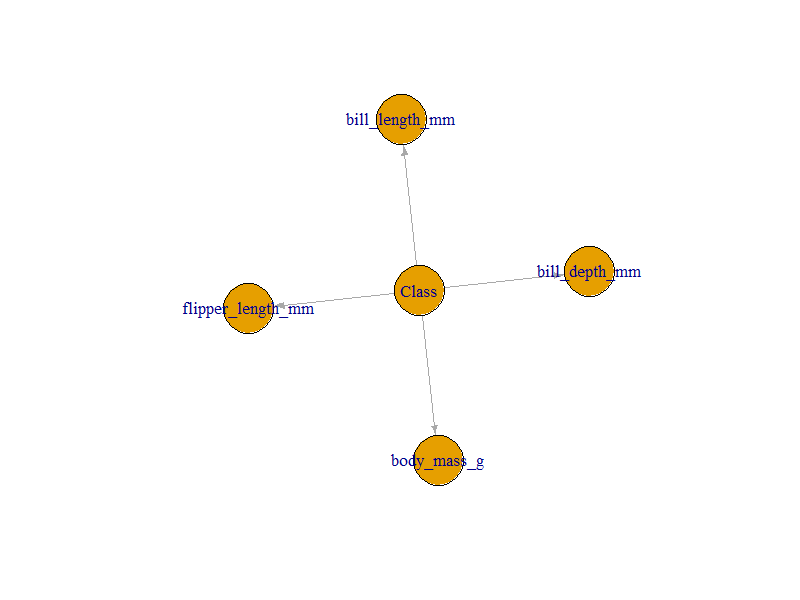
\includegraphics[width=0.4\textwidth]{IMG/2RED.png}
	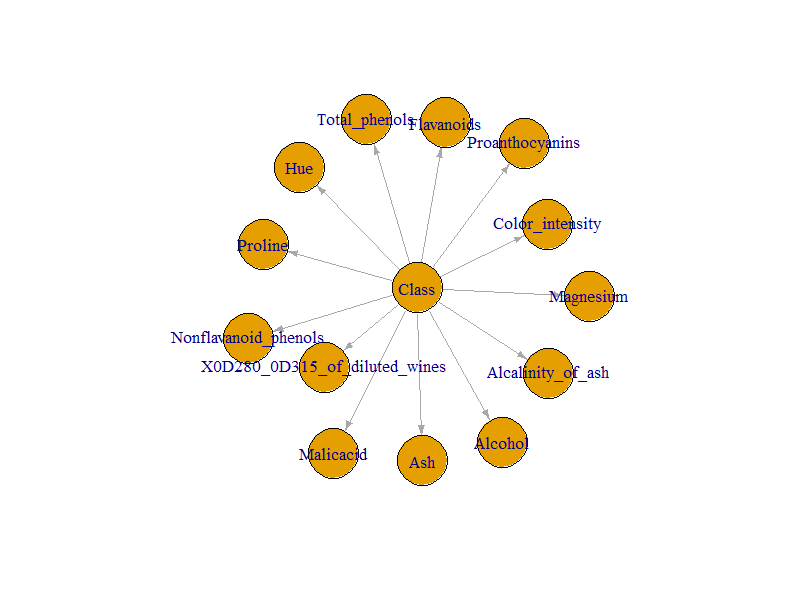
\includegraphics[width=0.4\textwidth]{IMG/3RED.png}\\[1ex]
	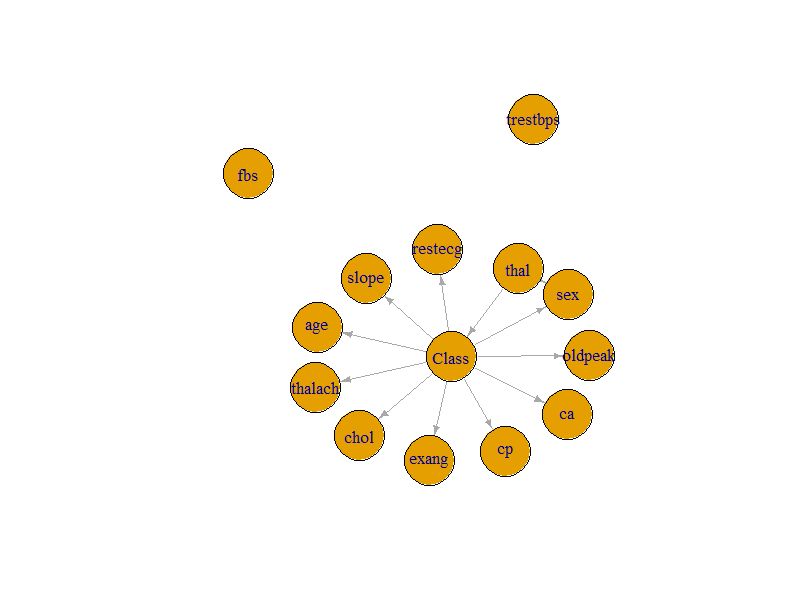
\includegraphics[width=0.4\textwidth]{IMG/4RED.png}
	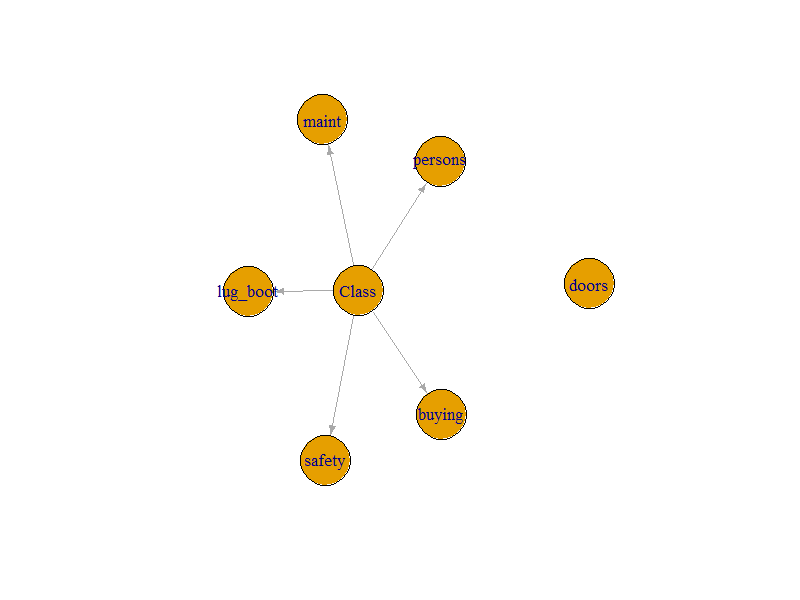
\includegraphics[width=0.4\textwidth]{IMG/5RED.png}
	\caption{Bayesian networks learned for the first five datasets: Iris, PalmerPenguin, Wine, HeartAttack, and CarsEvaluation.}
	\label{fig:networks_part1}
\end{figure}

\begin{figure}[htbp]
	\centering
	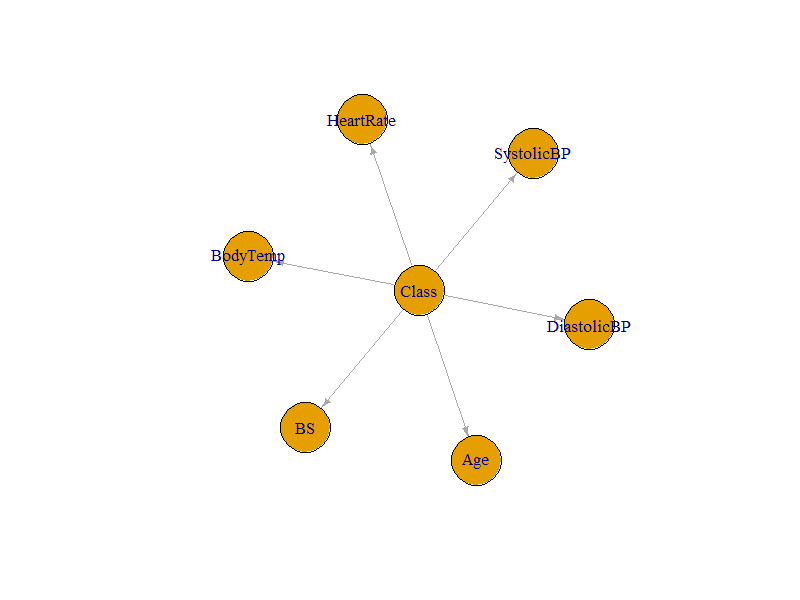
\includegraphics[width=0.4\textwidth]{IMG/6RED.png}
	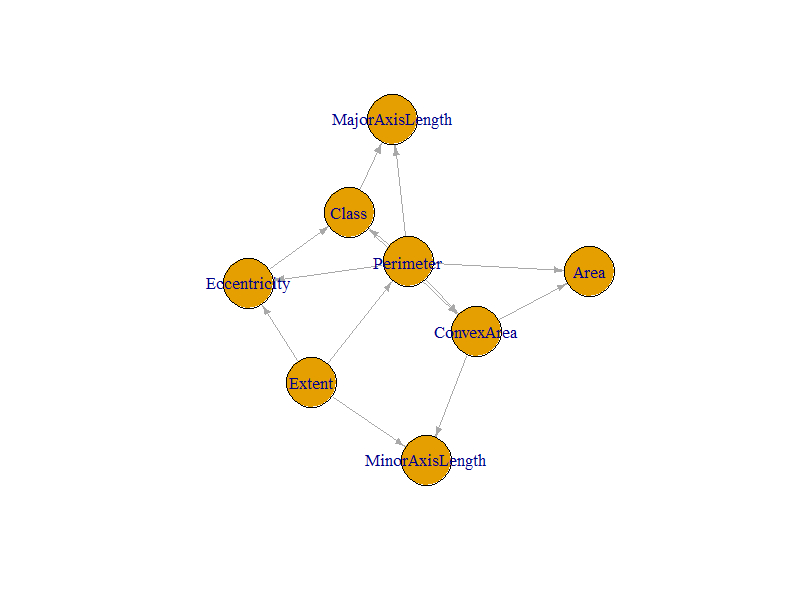
\includegraphics[width=0.4\textwidth]{IMG/7RED.png}
	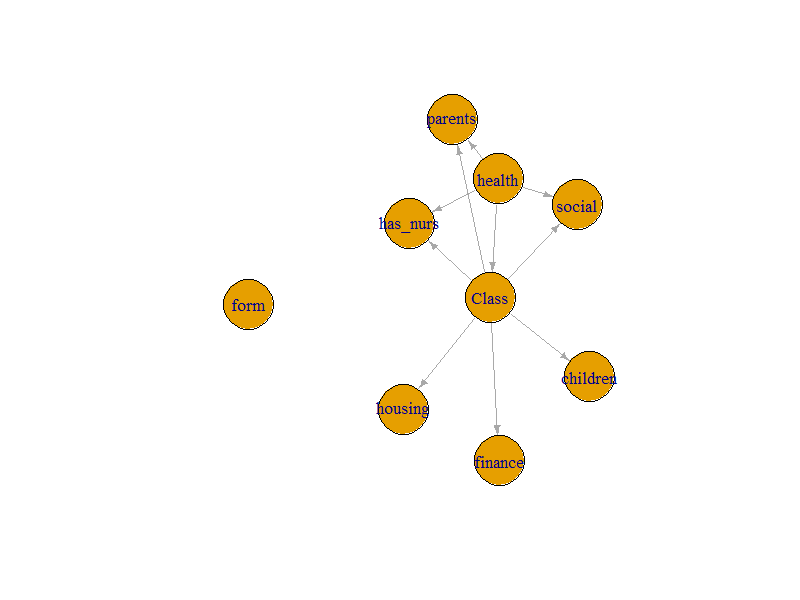
\includegraphics[width=0.4\textwidth]{IMG/8RED.png}\\[1ex]
	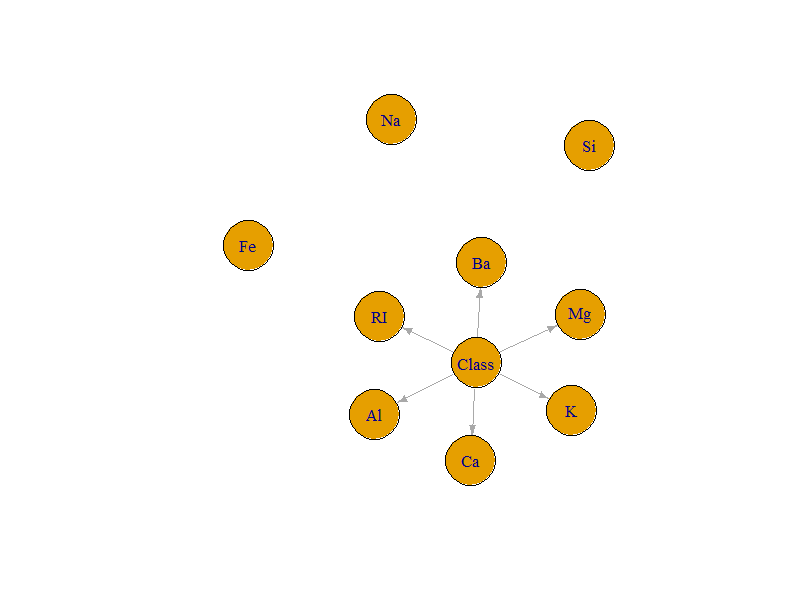
\includegraphics[width=0.4\textwidth]{IMG/9RED.png}
	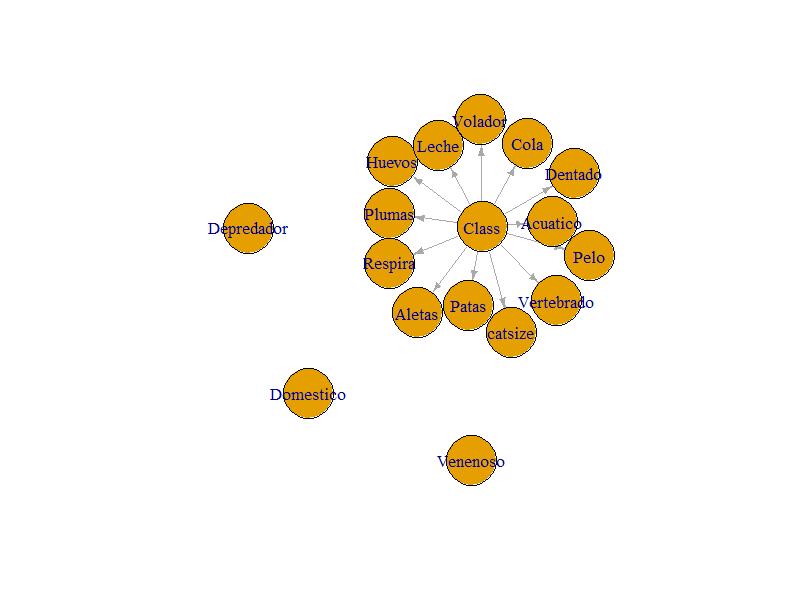
\includegraphics[width=0.4\textwidth]{IMG/10RED.png}
	\caption{Bayesian networks learned for the remaining datasets: MaternalHealthRisk, Raisins, Nurserys, Glass, and Zoo.}
	\label{fig:networks_part2}
\end{figure}

The learned structures for the ten UCI datasets (Figures~\ref{fig:networks_part1} and~\ref{fig:networks_part2}) generally exhibit a simplified pattern. In most cases, the networks resemble a Naïve Bayes configuration, with the class node connected directly to several input variables. Some variables remain unconnected, suggesting they were not informative under the MDL criterion. These results reflect compact, interpretable structures optimized for classification.



\newpage

\subsection{Structure Recovery on Synthetic Data from Gold Networks}

Table~\ref{tab:gold_networks} presents the performance of the genetic algorithm on seven benchmark (gold-standard) Bayesian networks. For each network, synthetic data was generated using the original structure and conditional probabilities. The learned structures were then compared against the originals using Kullback-Leibler divergence and Structural Hamming Distance (SHD).

Low KL divergence values (close to 0) indicate that the learned network models the data distribution similarly to the original. SHD values reflect the number of structural changes (additions, deletions, reversals) required to transform the learned structure into the true one.

It is worth noting that NA and Inf values in the Kullback-Leibler column result from structural inconsistencies detected by the bnlearn package when comparing certain networks. These inconsistencies typically arise when the learned structure differs significantly in conditional dependencies from the original network, causing the log-likelihood computation to fail or diverge.

\begin{table}[htbp]
	\centering
	\caption{Comparison with gold standard networks using Kullback-Leibler divergence and structural difference.}
	\begin{tabular}{lccccc}
		\hline
		\textbf{Gold Network} & \textbf{Nodes} & \textbf{Arcs} & \textbf{Parameters} & \textbf{Kullback-Leibler} & \textbf{Structural Difference} \\
		\hline
		ASIA       & 8  & 8  & 18   & 0.0000       & 8  \\
		CANCER     & 5  & 4  & 10   & 0.010997     & 4  \\
		EARTHQUAKE & 5  & 4  & 10   & NA           & 5  \\
		SACHS      & 11 & 17 & 178  & NA           & 8  \\
		SURVEY     & 6  & 6  & 21   & 0.031101     & 6  \\
		CHILD      & 20 & 25 & 230  & $\infty$     & 30 \\
		INSURANCE  & 27 & 52 & 1008 & 0.0000       & 82 \\
		\hline
	\end{tabular}
	\label{tab:gold_networks}
\end{table}


\newpage

\begin{figure}[H]
	\centering
	\begin{tabular}{ccc}
		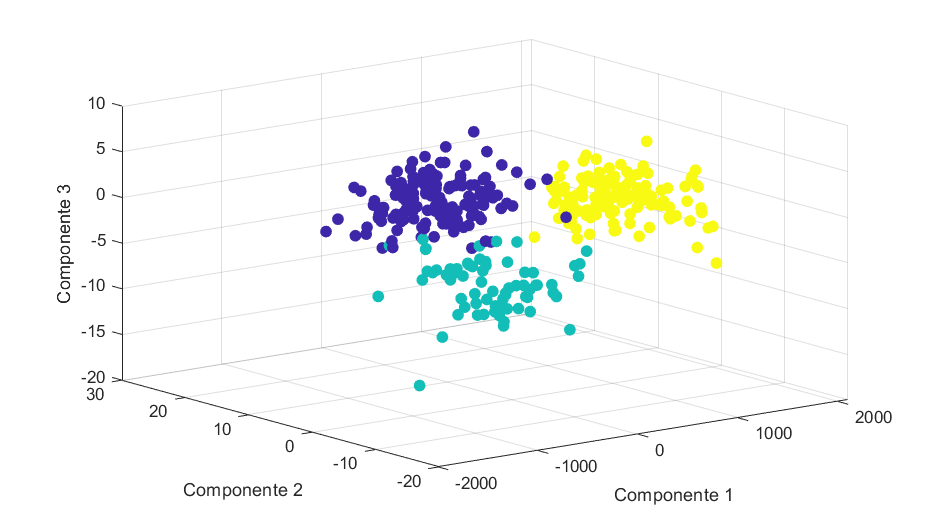
\includegraphics[width=0.3\textwidth]{IMG/G5.png} &
		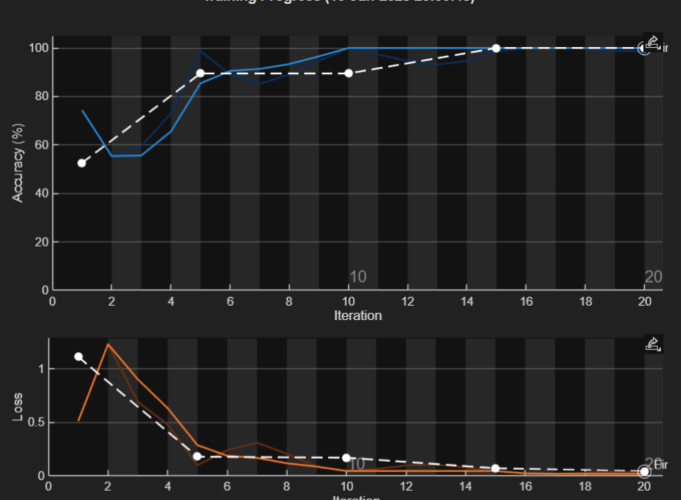
\includegraphics[width=0.3\textwidth]{IMG/G1.png} &
		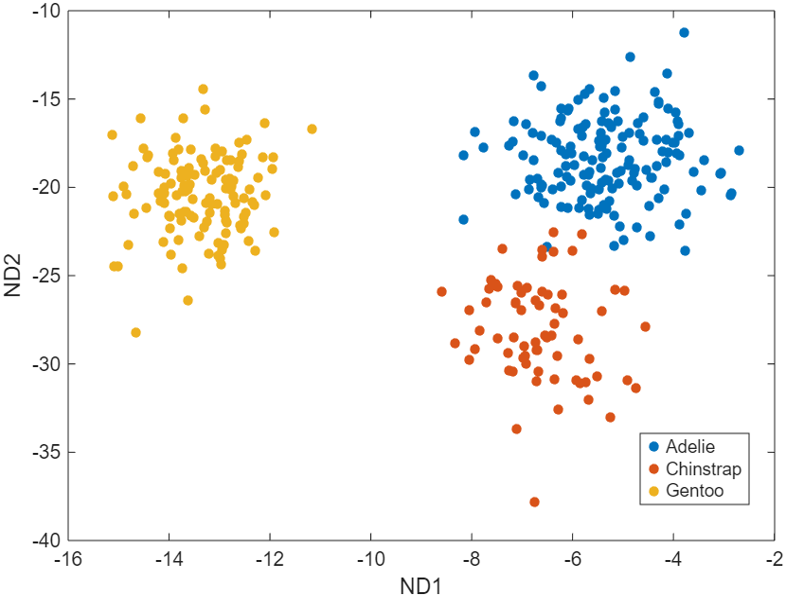
\includegraphics[width=0.3\textwidth]{IMG/G6.png} \\
		Gold Network: \textbf{SURVEY} & \textbf{ASIA} & \textbf{CHILD} \\
		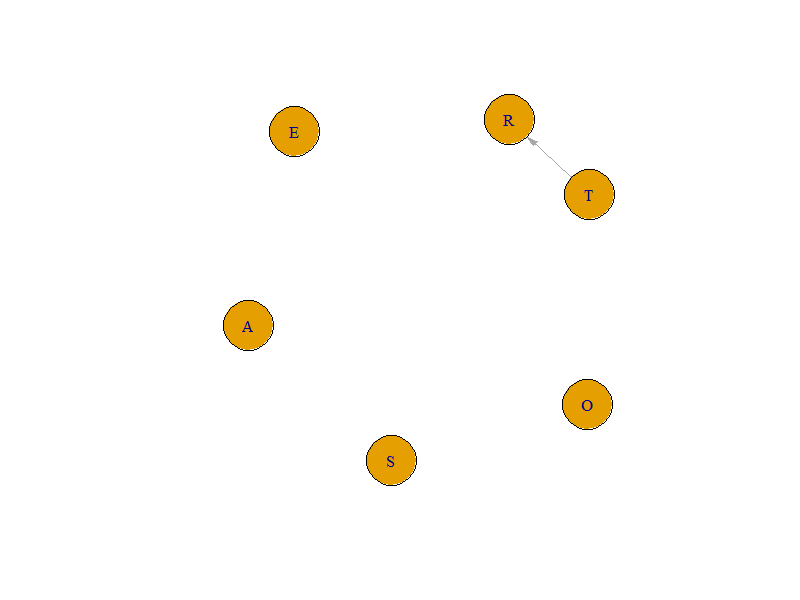
\includegraphics[width=0.3\textwidth]{IMG/1gr.png} &
		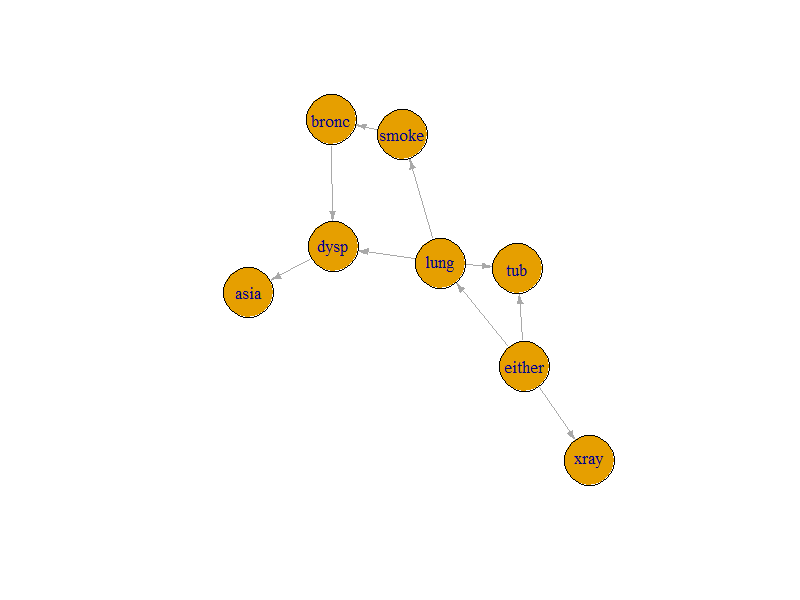
\includegraphics[width=0.3\textwidth]{IMG/2gr.png} &
		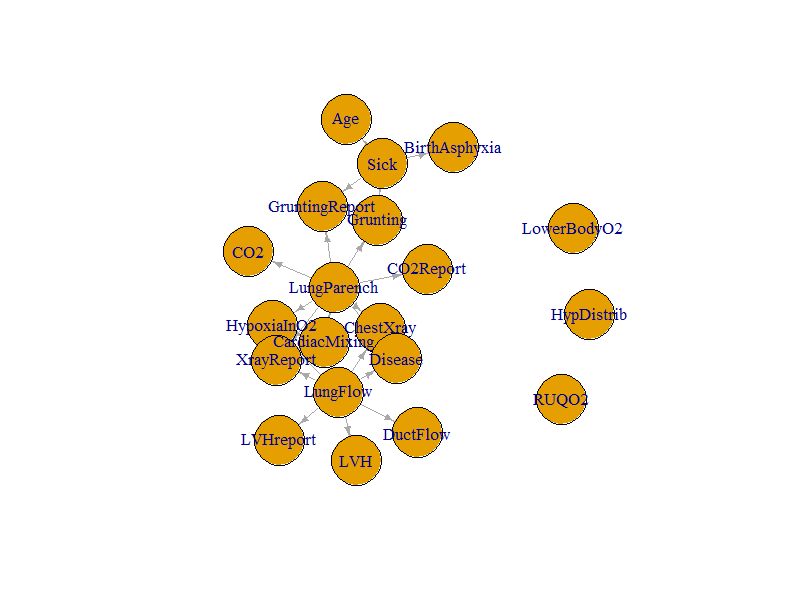
\includegraphics[width=0.3\textwidth]{IMG/3gr.png} \\
		Learned Network: \textbf{SURVEY} & \textbf{ASIA} & \textbf{CHILD} \\
		
		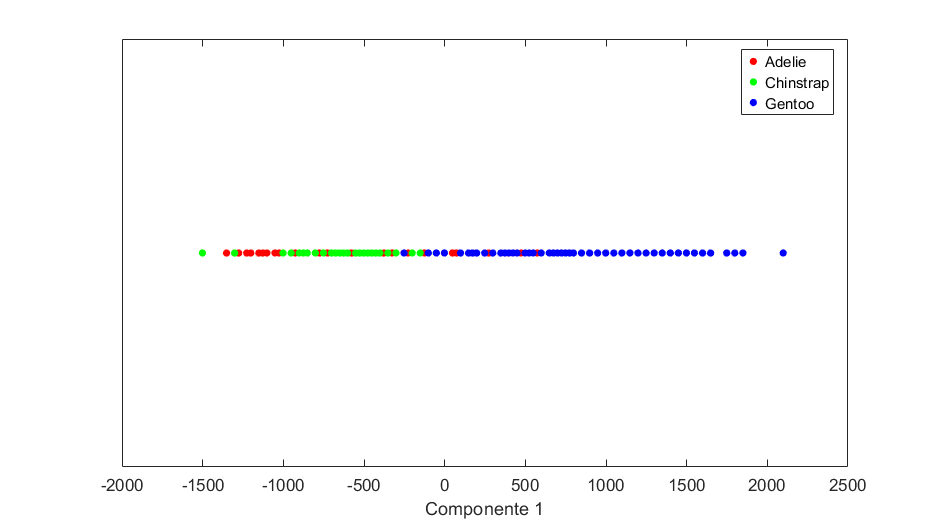
\includegraphics[width=0.3\textwidth]{IMG/G3.png} &
		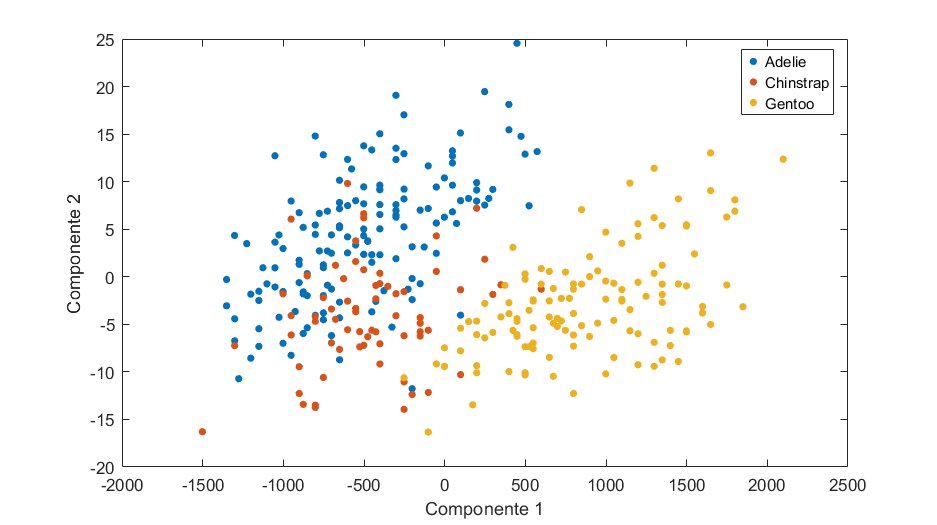
\includegraphics[width=0.3\textwidth]{IMG/G4.png} &
		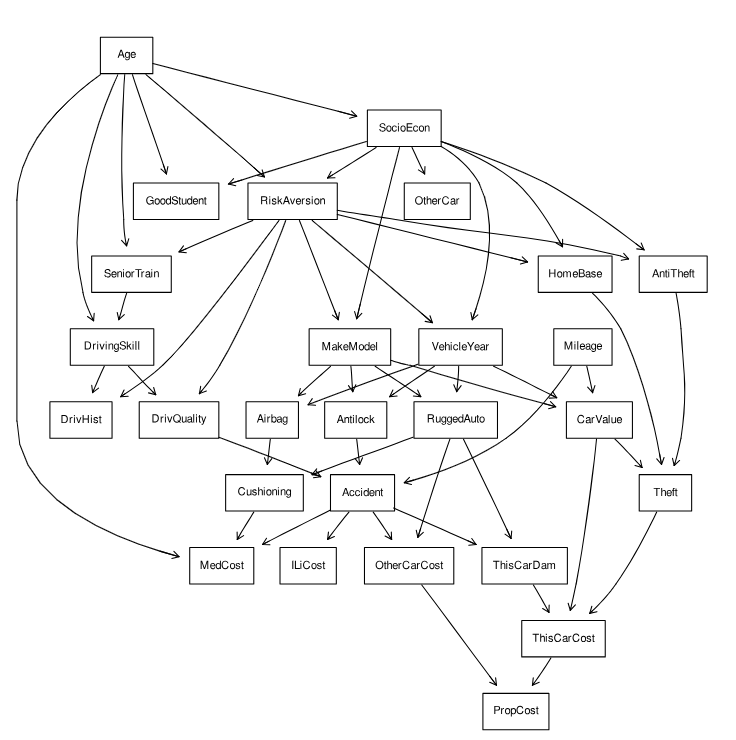
\includegraphics[width=0.3\textwidth]{IMG/G7.png} \\
		Gold Network: \textbf{EARTHQUAKE} & \textbf{SACHS} & \textbf{INSURANCE} \\
		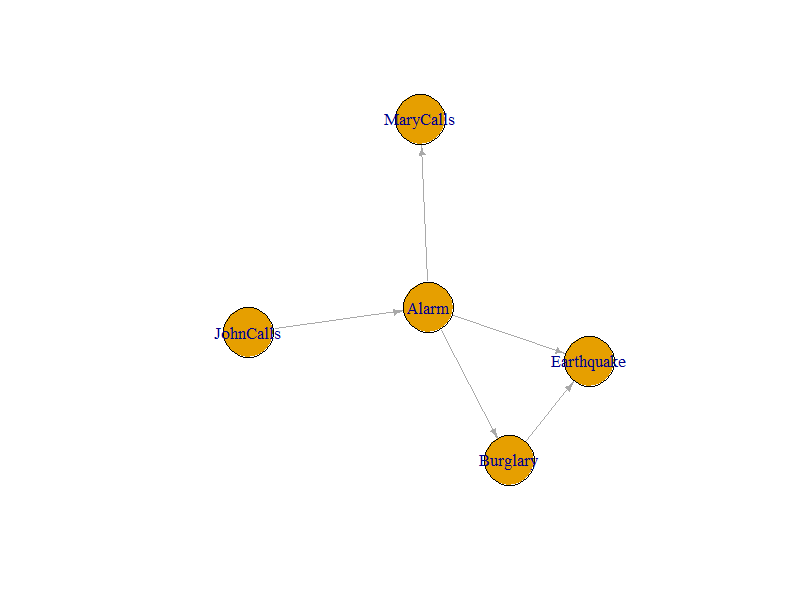
\includegraphics[width=0.3\textwidth]{IMG/4gr.png} &
		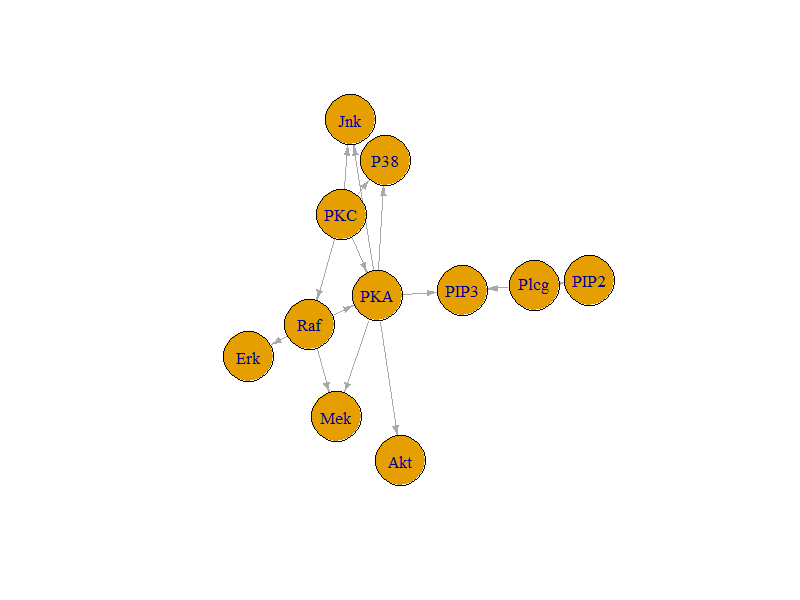
\includegraphics[width=0.3\textwidth]{IMG/5gr.png} &
		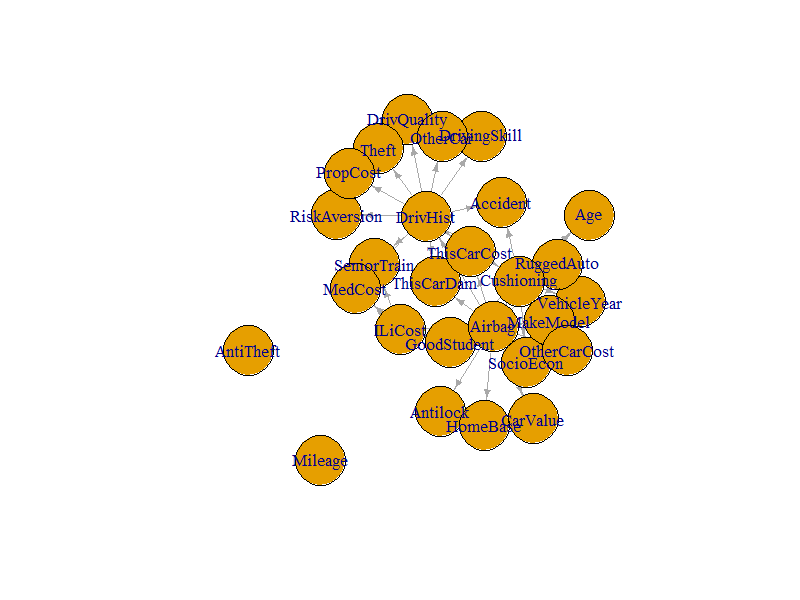
\includegraphics[width=0.3\textwidth]{IMG/6gr.png} \\
		Learned Network: \textbf{EARTHQUAKE} & \textbf{SACHS} & \textbf{INSURANCE} \\
		
		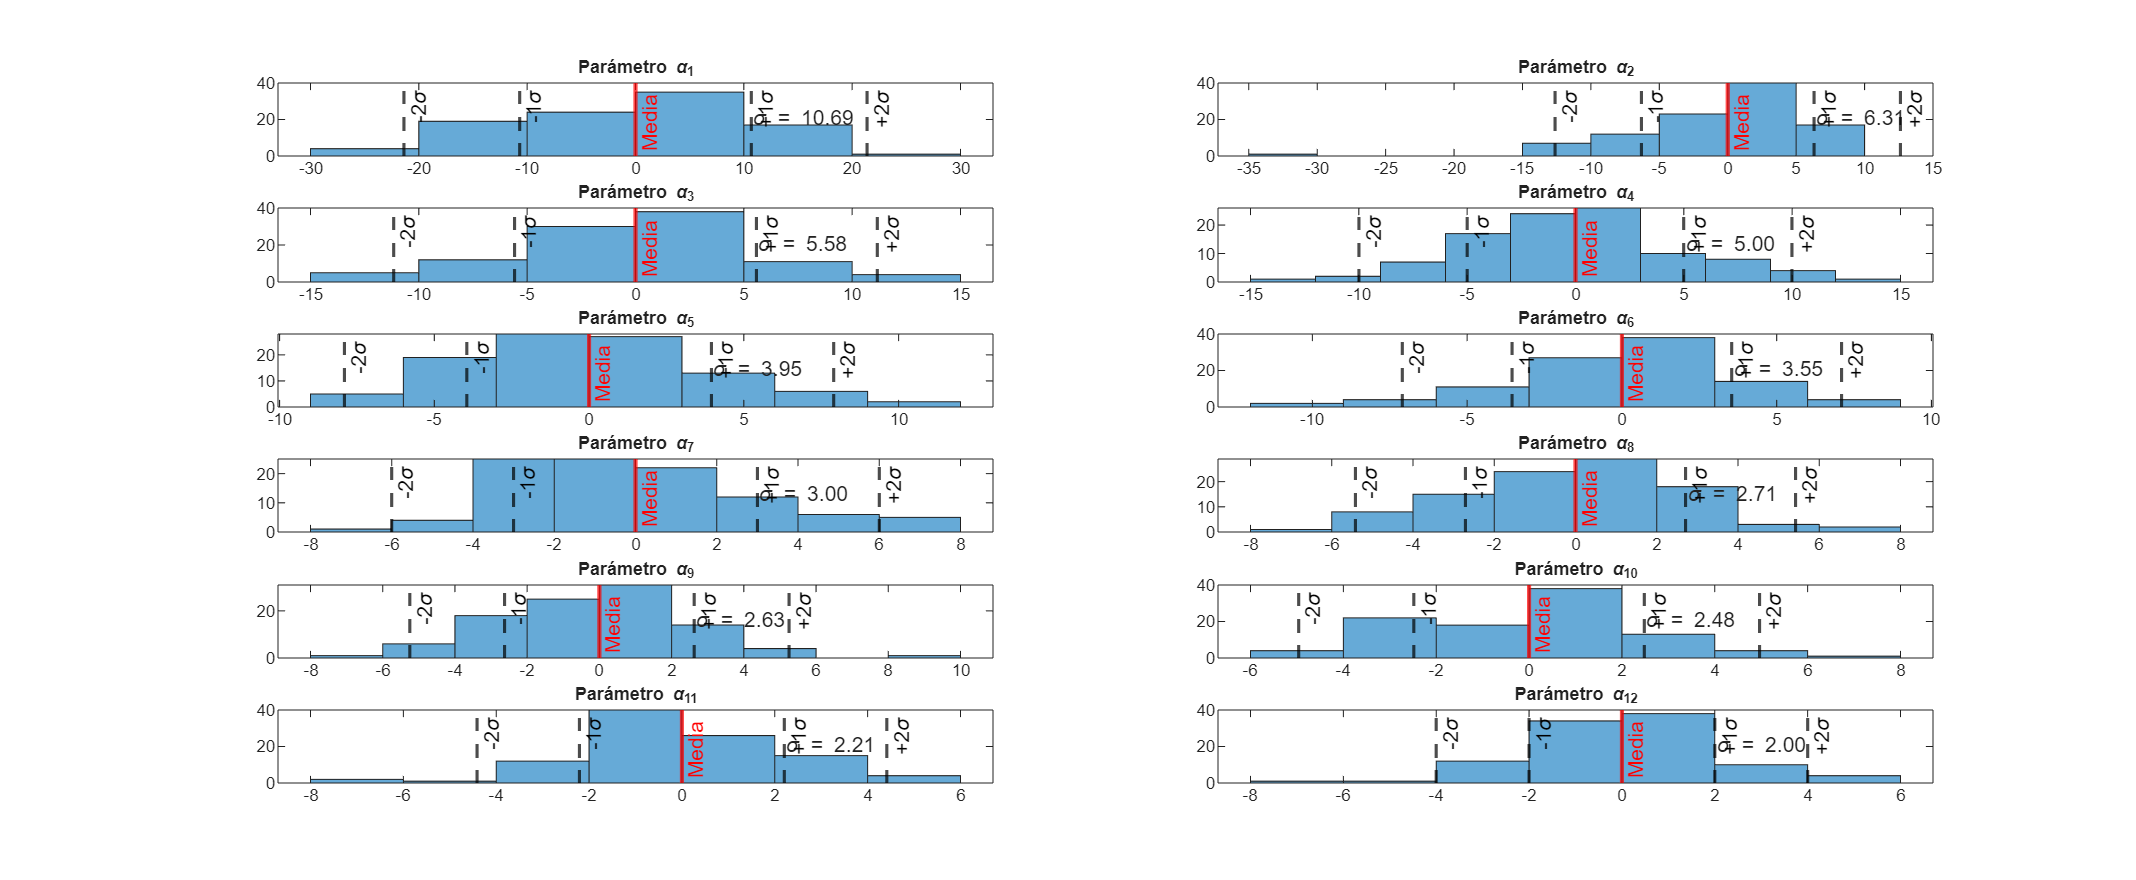
\includegraphics[width=0.3\textwidth]{IMG/G2.png} & & \\
		Gold Network: \textbf{CANCER} & & \\
		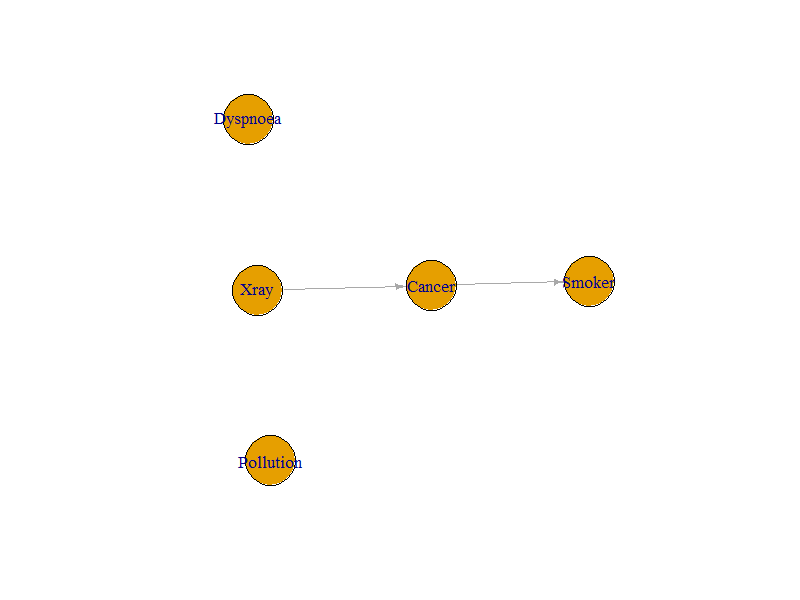
\includegraphics[width=0.3\textwidth]{IMG/7gr.png} & & \\
		Learned Network: \textbf{CANCER} & &
	\end{tabular}
	\caption{Visual comparison between gold standard and learned networks. Each pair of rows shows a gold network (top) and its corresponding learned structure (bottom).}
	\label{fig:network_comparison_ordered}
\end{figure}


\newpage

\subsection{Discusion}

The results obtained through the proposed genetic algorithm demonstrate its ability to discover Bayesian structures reasonably consistent with the data, even in varied domains with different complexity. In tests on real UCI sets, the model achieves high levels of accuracy, with acceptable execution times, especially on small to medium-sized datasets. On the other hand, when comparing with gold networks, it is observed that the algorithm is able to approximate similar structures, although in some cases significant deviations arise both in the Kullback-Leibler distance and in the structural difference.

A relevant observation is that the learned structures tend to form configurations close to the Naive Bayes classifier, which may indicate a preference of the algorithm for simpler solutions, penalized less by the MDL criterion. While this may be suitable for classificatory tasks, it also reveals a limitation in capturing deeper causal relationships or more complex conditional dependencies.

Furthermore, the algorithm's performance against larger networks and connectivity, such as CHILD or INSURANCE, suggests that there is room for improvement in exploring the structural space, possibly by incorporating more specific heuristics or additional constraints that better guide the evolutionary search.

\subsection{Conclusion and Future WorK}

This work presents a robust implementation of a genetic algorithm for Bayesian structure learning, achieving good results both in accuracy and modeling capacity on real and synthetic data. However, it is evident that the methodology can still benefit from improvements, especially to overcome its tendency to simple models and to identify more accurately complex relationships between variables.

Future work includes the integration of hybrid methods that combine evolutionary strategies with local search heuristics, as well as experimentation with new evaluation functions that are more sensitive to the global structure of the network, with the aim of increasing structural fidelity without sacrificing predictive capacity.

%
% ---- Bibliography ----
%
% BibTeX users should specify bibliography style 'splncs04'.
% References will then be sorted and formatted in the correct style.
%
% \bibliographystyle{splncs04}
% \bibliography{mybibliography}
%

\begin{thebibliography}{9}
	\bibitem{chickering1996learning}
	Chickering, D. M.: Learning Bayesian networks is NP-complete. In: Learning from data, pp. 121–130. Springer (1996)
	
	\bibitem{zhang2024bayesian}
	Zhang, Y., Zhuang, J., Jiang, J., Zhang, G., Qian, G.: Bayesian network structure learning: An improved genetic algorithm based on a new crossover operator. In: Lecture Notes in Computer Science, Springer (2024)
	
	\bibitem{sun2022bayesian}
	Sun, B., Zhou, Y.: Bayesian network structure learning with improved genetic algorithm. \textit{International Journal of Intelligent Systems}, \textbf{37}(9), 6023--6047 (2022)
	
	\bibitem{rosendo2022modelo}
	Rosendo, A., Toriz, E., Rodríguez, A.: Modelo adaptativo bayesiano basado en algoritmos evolutivos para la clasificación de datos. In: Congreso Nacional de Ingeniería (2022)
	
	\bibitem{scutari2010bnlearn}
	Scutari, M.: Learning Bayesian Networks with the \texttt{bnlearn} R Package. Journal of Statistical Software, \textbf{35}(3), 1--22 (2010). \url{https://doi.org/10.18637/jss.v035.i03}
	
	\bibitem{uci2024}
	Dua, D., Graff, C.: UCI Machine Learning Repository. University of California, Irvine, School of Information and Computer Sciences (2024). \url{https://archive.ics.uci.edu}
	
	
\end{thebibliography}

\end{document}
